\section{数制}

\begin{frame}\ft{\secname}
\begin{dingyi}[数制]
用一组固定的符号和统一的规则来表示数值的方法。
\end{dingyi}
\vspace{0.2in}

\red{常用的数制:}
\begin{AutoMultiColItemize}
\item 十进制
\item 二进制
\item 八进制
\item 十六进制
\end{AutoMultiColItemize}


在一种数制中,只能使用一组\red{固定的数字符号}来表示数目的大小。

\red{具体使用多少个数字符号来表示数目的大小,就称为该数制的基数。}
\end{frame}

\begin{frame}\ft{\secname}

\begin{table}
\begin{tabular}{ccccc}\hline
&基数&数字符号&最小数码&最大数码\\\hline
二进制(Binary)&2&0,1&0&1\\[.1in]
八进制(Octal)&8&0-7&0&7\\[.1in]
十进制(Decimal)&10&0-9&0&9\\[.1in]
十六进制(Hexadecimal)&16&0-9,A-F&0&F\\\hline
\end{tabular}
\end{table}

\end{frame}



\begin{frame}\ft{\secname}
{既然有不同的进制,那么在给出一个数时,需指明是什么数制里的数。}
\vspace{0.1in}

如:$(1010)_2,~(1010)_8,~(1010)_{10},~(1010)_{16}$所代表的数值就不同。\vspace{0.15in}

{除了用下标表示外,还可用后缀字母来表示数制。}
\vspace{0.1in}

如:1A4EH,~FEEDH,~BADH与$\mbox{(1A4E)}_{16},~\mbox{(FEED)}_{16},~\mbox{(BAD)}_{16}$的意义相同。
\end{frame}

\begin{frame}\ft{\secname}
\begin{figure}[h]
\centering
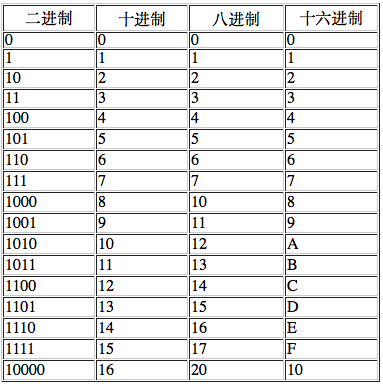
\includegraphics[width=3.in]{ch01/fig/shuzhi}
\end{figure}
\end{frame}

\begin{frame}\ft{进制}
{在数制中,N进制必须是逢N进一。}

\begin{itemize}
\item 十进制数:\red{逢十进一}。
\[
(1010)_{10}=1\times10^3+0\times10^2+1\times10^1+0\times10^0
\]
\item 二进制数:\red{逢二进一}。
\[
(1010)_{2}=1\times2^3+0\times2^2+1\times2^1+0\times2^0=(10)_{10}
\]
\item 八进制数:\red{逢八进一}。
\[
(1010)_{8}=1\times8^3+0\times8^2+1\times8^1+0\times8^0=(520)_{10}
\]
\item 十六进制数:\red{逢十六进一}。
\[
\mbox{(BAD)}_{16}=11\times16^2+10\times16^1+13\times16^0=(2989)_{10}
\]
\end{itemize}
\end{frame}

\begin{frame}\ft{二进制数的加法法则}

\[
\boxed{
\begin{array}{l}
0+0=0\\
0+1=1\\
1+0=1\\
1+1=10\\
1+1+1=10+1=11
\end{array}
}
\]

\begin{table}
\centering
\begin{tabular}{cD{.}{.}{3}}
&1011\\
+&1010\\
\hline
=&10101
\end{tabular}
\end{table}
\end{frame}

\begin{frame}\ft{二进制数的减法法则}

\[
\boxed{
\begin{array}{rl}
0-0=0&\\
1-0=1&\\
1-1=0&\\
0-1=1&\mbox{有借位,借1当$(10)_2$}\\
0-1-1=0&\mbox{有借位}\\
1-1-1=1&\mbox{有借位}\\
\end{array}
}
\]

\begin{table}
\centering
\begin{tabular}{cD{.}{.}{3}}
%&111110\\
&1~1~0~0~0~0\\
-&1~0~1~1~1\\
\hline
=&1~1~0~0~1
\end{tabular}
\end{table}
\end{frame}

\begin{frame}\ft{二进制的乘法法则}

\[\boxed{
\begin{array}{rr}
0\times0=0, & 
0\times1=0\\
1\times0=0, & 
1\times1=1\\
\end{array}
}
\]

\begin{table}
\centering
\begin{tabular}{cD{.}{.}{3}}
%&111110\\
&1~1~1~0\\
$\times$&0~1~1~0\\
\hline
&0~0~0~0\\
&1~1~1~0~~~\\
&1~1~1~0~~~~~\\
+&0~0~0~0~~~~~~~~\\
\hline
&1~0~1~0~1~0~0
\end{tabular}
\end{table}

\end{frame}
%
\begin{frame}\ft{二进制的除法法则}

\begin{figure}
\centering
\begin{tikzpicture}
\matrix[ampersand replacement=\&,matrix of math nodes,nodes={inner sep=0.2em}]{
    \& \& \& \&  \& 1 \& 1 \& 0 \& 1\\[4pt]
110 \& \sqrt{} \& |(a)|1\& 0 \& 0\& 1 \& 1 \& 1 \& |(b)| 0 \\
    \& - \&  |(c)| \&  1 \& 1\& |(d)|0  \&  \&  \&   \\[4pt]
    \&   \&   \&   \& 1\& 1  \& 1\&  \&   \\[4pt]
    \& - \&   \&   \& |(e)|1\& 1  \& |(f)|0\&  \&   \\[4pt]
    \&   \&   \&   \&  \&    \& 1\& 1\& 0  \\[4pt]
    \& - \&   \&   \&  \&    \& |(g)|1\& 1\& |(h)|0  \\[4pt]
    \&   \&   \&   \&  \&    \&  \&  \& 0  \\[4pt]
};
\draw[thick] (a.north west) -- (b.north east)
      (c.south west) -- (d.south east)
      (e.south west) -- (f.south east)
      (g.south west) -- (h.south east);

\end{tikzpicture}
\end{figure}
\end{frame}

\begin{frame}\ft{十进制数到二进制数的转换}

{(1)整数部分} 除2取余,直至商为0,最后将所得余数按逆序排列。 \vspace{0.1in}

\begin{figure}
\centering
\begin{tikzpicture}
\matrix[ampersand replacement=\&,matrix of math nodes,column sep=1ex,nodes={inner sep=0.2em}]{
    2  \& |(a)|  2 \& |(b)|3 \& \& \& \\[4pt]
    2  \& |(c)|  1 \& |(d)|1 \& \& \& \red{1}\\[4pt]
       \&        2 \& |(e)|5 \& \& \& \red{1}\\[4pt]
       \&        2 \& |(f)|2 \& \& \& \red{1}\\[4pt]
       \&        2 \& |(g)|1 \& \& \& \red{0}\\[4pt]
       \&          \&      0 \& \& \& \red{1}\\[4pt]
};
\draw[thick] (a.north west)--(a.south west)--(b.south east)
(c.north west)--(c.south west)--(d.south east)
(e.north west)--(e.south west)--(e.south east)
(f.north west)--(f.south west)--(f.south east)
(g.north west)--(g.south west)--(g.south east);

\end{tikzpicture}
\end{figure}
结果为
$
(23)_{10}=(10111)_2.
$
\end{frame}
%
\begin{frame}\ft{十进制数到二进制数的转换}

{(2)小数部分} 乘2取整数,若小数部分是5的倍数,则以最后小数部分为0为止,否则以约定的精确度为准,最后将所取整数按顺序排列。 \vspace{0.1in}

\begin{figure}
\centering
\begin{tikzpicture}
\matrix[ampersand replacement=\&,matrix of math nodes,column sep=1ex,nodes={inner sep=0.2em}]{
            \& 0 \& .\& 2\& 5      \& \&  \\[4pt]
|(a)|\times \&   \&  \&  \& |(b)|2 \& \&   \\[4pt]
            \& 0 \& .\& 5\& 0      \& \& \mbox{取整数位}0 \\[4pt]
|(c)|\times \&   \&  \&  \& |(d)|2 \& \&   \\[4pt]
            \& 1 \& .\& 0\& 0      \& \& \mbox{取整数位}1  \\[4pt]        
};
\draw[thick] (a.south west)--(b.south east)
(c.south west)--(d.south east);
\end{tikzpicture}
\end{figure}

结果为
$
(0.25)_{10}=(0.01)_2.
$

\end{frame}
%
\begin{frame}\ft{十进制数到二进制数的转换}
\begin{li}
将十进制数$125.24$转换为二进制数(取四位小数)。
\end{li}
\pause 

\begin{figure}
\begin{minipage}[t]{0.45\linewidth}
\centering
\begin{tikzpicture}[scale=0.8]
\matrix[ampersand replacement=\&,matrix of math nodes,column sep=1ex,nodes={inner sep=0.2em}]{
    2  \& |(a)|  1 \&       2 \& |(b)|5 \& \& \& \\[4pt]
    2  \& |(c)|  1 \&       6 \& |(d)|2 \& \& \& \red{1}\\[4pt]
       \&        2 \& |(e1)|3 \& |(e)|1 \& \& \& \red{0}\\[4pt]
       \&        2 \& |(f1)|1 \& |(f)|5 \& \& \& \red{1}\\[4pt]
       \&          \&       2 \& |(g)|7 \& \& \& \red{1}\\[4pt]
       \&          \&       2 \& |(h)|3 \& \& \& \red{1}\\[4pt]
       \&          \&       2 \& |(i)|1 \& \& \& \red{1}\\[4pt]       
       \&          \&         \&      0 \& \& \& \red{1}\\[4pt]
};
\draw[thick] (a.north west)--(a.south west)--(b.south east)
(c.north west)--(c.south west)--(d.south east)
(e1.north west)--(e1.south west)--(e.south east)
(f1.north west)--(f1.south west)--(f.south east)
(g.north west)--(g.south west)--(g.south east)
(h.north west)--(h.south west)--(h.south east)
(i.north west)--(i.south west)--(i.south east);

\end{tikzpicture}
\end{minipage}
\hfill
\begin{minipage}[t]{0.45\linewidth}
\centering
\begin{tikzpicture}[scale=0.8]
\matrix[ampersand replacement=\&,matrix of math nodes,column sep=1ex,nodes={inner sep=0.1em}]
{
            \& 0 \& .\& 2\& 4      \& \&  \\[4pt]
|(a)|\times \&   \&  \&  \& |(b)|2 \& \&   \\[4pt]
            \& 0 \& .\& 4\& 8      \& \& \mbox{取整数位}0 \\[4pt]
|(c)|\times \&   \&  \&  \& |(d)|2 \& \&   \\[4pt]
            \& 0 \& .\& 9\& 6      \& \& \mbox{取整数位}0  \\[4pt]
|(e)|\times \&   \&  \&  \& |(f)|2 \& \&   \\[4pt]
            \& 1 \& .\& 9\& 2      \& \& \mbox{取整数位}1  \\[4pt]                    
|(g)|\times \&   \&  \&  \& |(h)|2 \& \&   \\[4pt]
            \& 1 \& .\& 8\& 4      \& \& \mbox{取整数位}1  \\[4pt]            
};
\draw[thick] (a.south west)--(b.south east)
(c.south west)--(d.south east)
(e.south west)--(f.south east)
(g.south west)--(h.south east);
\end{tikzpicture}
\end{minipage}
\end{figure}
\pause 
结果为
$$
(125.24)_{10}=(1111101.0011)_2.
$$
\end{frame}
%
\begin{frame}\ft{二进制数到十进制数的转换}

{基本原理:} 
\begin{itemize}
\item 将二进制数从小数点开始,往左从$0$开始对各位进行正序编号,往右序号则分别为$-1,-2,-3,\cd$,直到最末位。\\[0.1in]
\item 然后分别将各位上的数乘以$2$的$k$次幂所得的值进行求和,其中$k$的值为各个位所对应的上述编号。
\end{itemize}
\end{frame}

\begin{frame}\ft{二进制数到十进制数的转换}
\begin{li}
将二进制数$1101.101$转换为十进制数(取四位小数)。
\end{li}
\pause 
$$
\begin{array}{rl}
& (1101.101)_2 \\[0.1in]
= & 1\times2^3+1\times2^2+0\times2^1+1\times2^0
+1\times2^{-1}+0\times2^{-2}+1\times2^{-3}\\[0.1in]
= & 8+4+1+0.5+0.125\\[0.1in]
= & 13.625
\end{array}
$$
\end{frame}
%
\begin{frame}\ft{二进制数到十六进制数的转换}

{基本原理:} 由于十六进制数基数是2的四次幂,所以一个二进制转换为十六进制,
\begin{itemize}
\item
如果是整数,只要从它的低位到高位每$4$位组成一组,然后将每组二进制数所对应的数用十六进制表示出来。\\[0.1in]
\item
如果有小数部分,则从小数点开始,分别向左右两边按照上述方法进行分组计算。
\end{itemize}
\end{frame}
%
\begin{frame}\ft{二进制数到十六进制数的转换}
\begin{li}
将二进制数$11~1010~1111~0001~0111$转换为十六进制数。
\end{li}
\pause 
\begin{table}
\centering
\begin{tabular}{cccccc}\hline
二进制数&$11$&$1010$&$1111$&$0001$&$0111$\\[0.1in]
十六进制数&$3$&$A$&$F$&$1$&$7$\\ \hline
\end{tabular}
\end{table}
结果为
$$
(11~1010~1111~0001~0111)_2=(3AF17)_{16}
$$
\end{frame}
%
%
